\documentclass[10pt,a4paper,landscape]{article}
\usepackage{geometry}
\usepackage{tikz}
\usepackage[most]{tcolorbox}
\usepackage{amsmath}
\usepackage{amsfonts}
\usepackage{amssymb}
\usepackage{graphicx}
\usepackage{xcolor}
\usepackage{hyperref}
\usepackage{multirow}
\usepackage{multicol}
\usepackage{wasysym}
\usepackage{fontspec}
\usepackage{unicode-math}
\usepackage{enumitem}

% Modern color scheme
\definecolor{primary}{RGB}{41, 128, 185}      % Blue
\definecolor{secondary}{RGB}{39, 174, 96}     % Green
\definecolor{accent}{RGB}{192, 57, 43}        % Red
\definecolor{neutral}{RGB}{52, 73, 94}        % Dark blue-gray
\definecolor{light}{RGB}{236, 240, 241}       % Light gray
\definecolor{boxbg}{RGB}{245, 247, 250}       % Very light blue-gray

% font setup
\setmainfont{IBM Plex Serif}
\setsansfont{IBM Plex Sans}
\setmonofont{IBM Plex Mono}
\setmathfont{STIX Two Math}

% Tight layout with less space wastage
\setlength{\parindent}{0pt}
\setlength{\parskip}{0.5pt}
\setlength{\columnsep}{8pt}
\setlength{\marginparwidth}{0pt}
\setlength{\marginparsep}{0pt}

% Page layout - maximize space
\geometry{top=0.3in, bottom=0.3in, left=0.3in, right=0.3in}

% Custom commands for better formatting
\newcommand{\sheader}[1]{%
  \vspace{1mm}
  \noindent{\color{primary}\textbf{\large #1}}
  \vspace{-0.5mm}\\
  \rule{\linewidth}{0.8pt}
  \vspace{0mm}
}

\newcommand{\ssubheader}[1]{%
  \vspace{0.5mm}
  \noindent{\color{secondary}\textbf{\normalsize #1}}
  \vspace{0mm}
}

\newcommand{\alert}[1]{\textcolor{accent}{\textbf{#1}}}
\newcommand{\note}[1]{\textcolor{neutral}{\textit{#1}}}

% Unified formula environment
\newtcolorbox{formula}[2][]{
  enhanced jigsaw,
  colback=boxbg,
  colframe=primary!70,
  fonttitle=\bfseries\small,
  coltitle=neutral,
  boxrule=0.7pt,
  sharp corners,
  top=1pt,
  bottom=1pt,
  left=2pt,
  right=2pt,
  before skip=2pt,
  after skip=2pt,
  title=#2,
  label=#1
}

% Slim code environment
\newtcolorbox{codebox}[2][]{
  enhanced jigsaw,
  colback=light,
  colframe=secondary!70,
  fonttitle=\bfseries\small,
  coltitle=neutral,
  boxrule=0.7pt,
  sharp corners,
  top=1pt,
  bottom=1pt,
  left=2pt,
  right=2pt,
  before skip=2pt,
  after skip=2pt,
  title=#2,
  label=#1
}

\begin{document}

\begin{multicols}{3}

  %----------------------------------------------------------------------------------------
  % FDM SECTION - THEORY
  %----------------------------------------------------------------------------------------

  \sheader{Finite Difference Methods (FDM)}

  \ssubheader{Core Differentiation Operators}

  \begin{formula}{Basic Operators}
    $\Delta_h u(x) = u(x+h) - u(x)$ \hfill (Forward) \\
    $\nabla_h u(x) = u(x) - u(x-h)$ \hfill (Backward) \\
    $\delta_h u(x) = u(x+h) - u(x-h)$ \hfill (Central) \\
    $\delta_h^2 u(x) = u(x+h) - 2u(x) + u(x-h)$ \hfill (2nd order)
  \end{formula}

  \begin{formula}{Approximations with Error Terms}
    $\frac{\Delta_h u(x)}{h} = u'(x) + \frac{h}{2}u''(x) + O(h^2)$ \\
    $\frac{\nabla_h u(x)}{h} = u'(x) - \frac{h}{2}u''(x) + O(h^2)$ \\
    $\frac{\delta_h u(x)}{2h} = u'(x) + O(h^2)$ \\
    $\frac{\delta_h^2 u(x)}{h^2} = u''(x) + O(h^2)$
  \end{formula}

  \begin{center}
    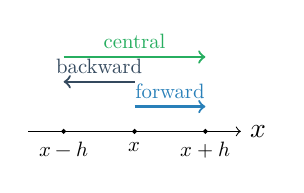
\begin{tikzpicture}[scale=0.45]
      % Number line
      \draw[->] (0,0) -- (6,0) node[right] {$x$};

      % Points and labels - simplified
      \foreach \x/\label in {1/x-h, 3/x, 5/x+h} {
          \filldraw[black] (\x,0) circle (1.5pt);
          \node[below,scale=0.75] at (\x,-0.1) {$\label$};
        }

      % Simplified arrows
      \draw[primary, ->, thick] (3,0.7) -- (5,0.7) node[midway, above, scale=0.75] {forward};
      \draw[neutral, ->, thick] (3,1.4) -- (1,1.4) node[midway, above, scale=0.75] {backward};
      \draw[secondary, ->, thick] (1,2.1) -- (5,2.1) node[midway, above, scale=0.75] {central};
    \end{tikzpicture}
  \end{center}

  \ssubheader{Higher-Order Formulas}

  \begin{formula}{$4^{th}$ Order Central Differences}
    $u'(x) \approx \frac{-u(x+2h) + 8u(x+h) - 8u(x-h) + u(x-2h)}{12h}$ \\[0.3em]
    $u''(x) \approx \frac{-u(x+2h) + 16u(x+h) - 30u(x) + 16u(x-h) - u(x-2h)}{12h^2}$
  \end{formula}

  \begin{formula}{Compact FD Coefficients}
    \small
    \begin{tabular}{|c|c|ccccc|}
      \hline
      Deriv.                 & Accuracy & \multicolumn{5}{c|}{Stencil Points}                             \\
                             &          & -2                                  & -1   & 0    & +1  & +2    \\
      \hline
      \multirow{3}{*}{$f'$}  & $O(h)$   & -                                   & -    & -1   & 1   & -     \\
                             & $O(h^2)$ & -                                   & -1/2 & 0    & 1/2 & -     \\
                             & $O(h^4)$ & 1/12                                & -2/3 & 0    & 2/3 & -1/12 \\
      \hline
      \multirow{2}{*}{$f''$} & $O(h^2)$ & -                                   & 1    & -2   & 1   & -     \\
                             & $O(h^4)$ & -1/12                               & 4/3  & -5/2 & 4/3 & -1/12 \\
      \hline
    \end{tabular}
  \end{formula}

  \ssubheader{Stability Analysis}

  \begin{formula}{von Neumann Analysis}
    \textbf{Ansatz:} $u_j^n = \xi^n e^{ij\theta}$ where $\xi = \xi(\theta)$ \\
    \textbf{Stability condition:} $|\xi(\theta)| \leq 1$ for all $\theta \in [-\pi, \pi]$ \\
    \textbf{Plotting method:} Graph $|\xi(\theta)|$ vs $\theta$ for fixed $\frac{\Delta t}{\Delta x}$
  \end{formula}

  \begin{formula}{Matrix Stability}
    For $\vec{u}^{n+1} = A\vec{u}^n$, stability requires: \\
    $\rho(A) \leq 1$ (spectral radius condition) \\[0.3em]
    \textbf{Types of stability:} \\
    $\bullet$ $\rho(A) < 1$: asymptotically stable \\
    $\bullet$ $\rho(A) = 1$ (simple): neutrally stable \\
    $\bullet$ $\rho(A) > 1$: unstable
  \end{formula}

  \begin{formula}{CFL Condition Summary}
    \textbf{Advection equation} $u_t + au_x = 0$: \\
    $C = \frac{|a|\Delta t}{\Delta x} \leq 1$ \\[0.3em]

    \textbf{Diffusion equation} $u_t = \alpha u_{xx}$: \\
    $r = \frac{\alpha \Delta t}{\Delta x^2} \leq \frac{1}{2}$ \\[0.3em]

    \textbf{2D Advection:} \\
    $\Delta t \left(\frac{|u_x|}{\Delta x} + \frac{|u_y|}{\Delta y}\right) \leq 1$ \\[0.3em]

    \textbf{2D Diffusion:} \\
    $\alpha\Delta t \left(\frac{1}{\Delta x^2} + \frac{1}{\Delta y^2}\right) \leq \frac{1}{2}$
  \end{formula}

  \begin{center}
    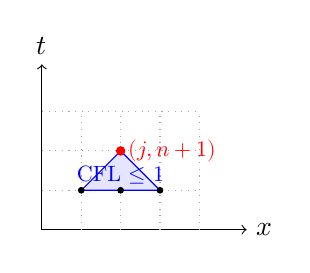
\begin{tikzpicture}[scale=0.5]
      % x/t grid
      \draw[->] (0,0) -- (5.2,0) node[right] {$x$};
      \draw[->] (0,0) -- (0,4.2) node[above] {$t$};

      % Grid lines
      \foreach \x in {1,2,...,4} {
          \draw[dotted, gray!70] (\x,0) -- (\x,3);
        }
      \foreach \y in {1,2,3} {
          \draw[dotted, gray!70] (0,\y) -- (4,\y);
        }

      % Domain of dependence
      \draw[blue, fill=blue!10] (2,2) -- (1,1) -- (3,1) -- cycle;
      \node[blue, scale=0.8] at (2,1.4) {CFL $\leq$ 1};

      % Current point
      \filldraw[red] (2,2) circle (3pt);
      \node[red, right, scale=0.8] at (2,2) {$(j,n+1)$};

      % Previous points
      \filldraw[black] (1,1) circle (2pt);
      \filldraw[black] (2,1) circle (2pt);
      \filldraw[black] (3,1) circle (2pt);
    \end{tikzpicture}
  \end{center}

  %----------------------------------------------------------------------------------------
  % FDM SECTION - APPLICATION
  %----------------------------------------------------------------------------------------

  \sheader{FDM Step-by-Step Process}

  \begin{codebox}{Solving Elliptic PDEs (Poisson)}{elliptic-steps}
    1. \textbf{Discretize domain}: $x_i = a + i\Delta x$, $y_j = b + j\Delta y$ \\
    2. \textbf{Discretize operators}: e.g., $\nabla^2 u \approx \frac{u_{i+1,j} + u_{i-1,j} + u_{i,j+1} + u_{i,j-1} - 4u_{i,j}}{h^2}$ \\
    3. \textbf{Apply boundary conditions}: Modify equations at boundary nodes \\
    4. \textbf{Form linear system}: $AU = b$ \\
    5. \textbf{Solve}: Direct or iterative method \\
    6. \textbf{Analyze error}: Compute $\mathcal{O}(h^p)$ convergence rate
  \end{codebox}

  \begin{formula}{2D Poisson Equation}
    \textbf{PDE:} $-\nabla^2 u = f$ in $\Omega$, $u = g$ on $\partial\Omega$ \\[0.3em]
    \textbf{5-point stencil:}
    $-\frac{u_{i+1,j} + u_{i-1,j} + u_{i,j+1} + u_{i,j-1} - 4u_{i,j}}{h^2} = f_{i,j}$ \\[0.3em]
    \textbf{Matrix form:} $AU = F$ with $A$ pentadiagonal
  \end{formula}

  \begin{center}
    \small
    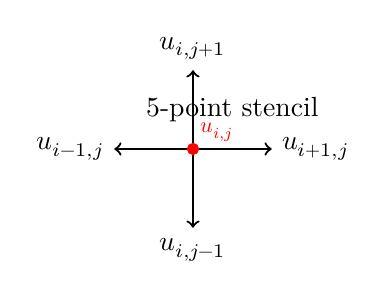
\begin{tikzpicture}[scale=0.5]
      % 5-point stencil
      \draw[->, thick] (0,0) -- (0,2) node[above] {$u_{i,j+1}$};
      \draw[->, thick] (0,0) -- (2,0) node[right] {$u_{i+1,j}$};
      \draw[->, thick] (0,0) -- (0,-2) node[below] {$u_{i,j-1}$};
      \draw[->, thick] (0,0) -- (-2,0) node[left] {$u_{i-1,j}$};
      \filldraw[red] (0,0) circle (4pt) node[above right, scale=0.8] {$u_{i,j}$};
      \node at (1,1) {5-point stencil};
    \end{tikzpicture}
  \end{center}

  \begin{codebox}{Solving Parabolic PDEs (Heat)}{parabolic-steps}
    1. \textbf{Discretize}: $x_i = a + i\Delta x$, $t_n = n\Delta t$ \\
    2. \textbf{Choose scheme}:
    - Explicit (FTCS): $\frac{u_i^{n+1} - u_i^n}{\Delta t} = \alpha \frac{u_{i+1}^n - 2u_i^n + u_{i-1}^n}{\Delta x^2}$ \\
    - Implicit (BTCS): $\frac{u_i^{n+1} - u_i^n}{\Delta t} = \alpha \frac{u_{i+1}^{n+1} - 2u_i^{n+1} + u_{i-1}^{n+1}}{\Delta x^2}$ \\
    - Crank-Nicolson (CN): Average of FTCS and BTCS \\
    3. \textbf{Apply conditions}: Initial and boundary \\
    4. \textbf{Stability check}: $r = \frac{\alpha \Delta t}{\Delta x^2} \leq \frac{1}{2}$ (FTCS) \\
    5. \textbf{Time-stepping}: March forward in time
  \end{codebox}

  \begin{formula}{Heat Equation Schemes}
    \textbf{Heat equation:} $u_t = \alpha u_{xx}$ \\[0.3em]
    \textbf{FTCS (Explicit):}
    $\frac{u_i^{n+1} - u_i^n}{\Delta t} = \alpha \frac{u_{i+1}^n - 2u_i^n + u_{i-1}^n}{\Delta x^2}$ \\[0.3em]
    \textbf{BTCS (Implicit):}
    $\frac{u_i^{n+1} - u_i^n}{\Delta t} = \alpha \frac{u_{i+1}^{n+1} - 2u_i^{n+1} + u_{i-1}^{n+1}}{\Delta x^2}$ \\[0.3em]
    \textbf{Crank-Nicolson:}
    $\frac{u_i^{n+1} - u_i^n}{\Delta t} = \frac{\alpha}{2} \left(\frac{u_{i+1}^{n+1} - 2u_i^{n+1} + u_{i-1}^{n+1}}{\Delta x^2} + \frac{u_{i+1}^n - 2u_i^n + u_{i-1}^n}{\Delta x^2}\right)$
  \end{formula}

  \begin{formula}{Stability for Heat Equation}
    \begin{tabular}{|c|c|c|c|}
      \hline
      \textbf{Scheme} & \textbf{Stability}   & \textbf{Accuracy}           & \textbf{Effort} \\
      \hline
      FTCS            & $r \leq \frac{1}{2}$ & $O(\Delta t, \Delta x^2)$   & Low             \\
      BTCS            & Unconditional        & $O(\Delta t, \Delta x^2)$   & Medium          \\
      CN              & Unconditional        & $O(\Delta t^2, \Delta x^2)$ & High            \\
      \hline
    \end{tabular}
  \end{formula}

  \begin{codebox}{Solving Hyperbolic PDEs (Wave)}{hyperbolic-steps}
    1. \textbf{Discretize}: $x_i = a + i\Delta x$, $t_n = n\Delta t$ \\
    2. \textbf{Choose scheme}: Consider characteristics \\
    3. \textbf{Apply conditions}: Initial and boundary \\
    4. \textbf{Stability check}: $C = \frac{c\Delta t}{\Delta x} \leq 1$ \\
    5. \textbf{Time-stepping}: Use multi-level methods
  \end{codebox}

  \begin{formula}{Transport Equation Schemes}
    \textbf{Transport equation:} $u_t + au_x = 0$ \\[0.3em]
    \textbf{Upwind (for $a > 0$):}
    $\frac{u_i^{n+1} - u_i^n}{\Delta t} + a\frac{u_i^n - u_{i-1}^n}{\Delta x} = 0$ \\[0.3em]
    \textbf{Lax-Friedrichs:}
    $\frac{u_i^{n+1} - \frac{1}{2}(u_{i+1}^n + u_{i-1}^n)}{\Delta t} + a\frac{u_{i+1}^n - u_{i-1}^n}{2\Delta x} = 0$ \\[0.3em]
    \textbf{Lax-Wendroff:}
    $\frac{u_i^{n+1} - u_i^n}{\Delta t} + a\frac{u_{i+1}^n - u_{i-1}^n}{2\Delta x} = \frac{a^2\Delta t}{2}\frac{u_{i+1}^n - 2u_i^n + u_{i-1}^n}{\Delta x^2}$
  \end{formula}

  \begin{formula}{Stability for Transport Equation}
    \begin{tabular}{|l|l|l|l|}
      \hline
      \textbf{Scheme} & \textbf{Stab.} & \textbf{Ord.} & \textbf{Prop.}    \\
      \hline
      Upwind          & $C \leq 1$     & 1             & Diffusive         \\
      Lax-Friedrichs  & $C \leq 1$     & 1             & Very diffusive    \\
      Lax-Wendroff    & $C \leq 1$     & 2             & Dispersive        \\
      Leapfrog        & $C \leq 1$     & 2             & Neutral, unstable \\
      \hline
    \end{tabular}
  \end{formula}

  %----------------------------------------------------------------------------------------
  % FEM SECTION - THEORY
  %----------------------------------------------------------------------------------------
  \sheader{Finite Element Methods (FEM)}
  \ssubheader{Key Concepts}
  \begin{formula}{Weak Formulation}
    \textbf{Strong form:} Find $u$ such that $Lu = f$ \\[0.3em]
    \textbf{Weak form:} Find $u \in V$ such that \\
    $a(u,v) = F(v) \quad \forall v \in V$ \\[0.3em]
    where $a(u,v)$ is a bilinear form and $F(v)$ is a linear functional
  \end{formula}

  \begin{formula}{From Strong to Weak Form}
    For $-\Delta u = f$ in $\Omega$ with $u=0$ on $\partial\Omega$: \\[0.3em]
    1. Multiply by test function $v \in V$: $-\int_\Omega v\Delta u \, dx = \int_\Omega vf \, dx$ \\
    2. Apply integration by parts: $\int_\Omega \nabla v \cdot \nabla u \, dx - \int_{\partial\Omega} v\frac{\partial u}{\partial n} \, ds = \int_\Omega vf \, dx$ \\
    3. Use $v=0$ on $\partial\Omega$: $\int_\Omega \nabla v \cdot \nabla u \, dx = \int_\Omega vf \, dx$
  \end{formula}

  \begin{formula}{Galerkin Method}
    \textbf{1. Choose finite-dimensional subspace} $V_h \subset V$ \\[0.3em]
    \textbf{2. Approximate:} $u \approx u_h = \sum_{j=1}^n c_j \phi_j$ \\[0.3em]
    \textbf{3. Form discrete problem:} Find $u_h \in V_h$ such that \\
    $a(u_h,v_h) = F(v_h) \quad \forall v_h \in V_h$ \\[0.3em]
    \textbf{4. Choose test functions:} $v_h = \phi_i$ for $i=1,\ldots,n$ \\[0.3em]
    \textbf{5. Get linear system:} $\mathbf{K}\mathbf{c} = \mathbf{F}$ where \\
    $K_{ij} = a(\phi_j,\phi_i)$ and $F_i = F(\phi_i)$
  \end{formula}

  \ssubheader{Function Spaces}

  \begin{formula}{Sobolev Spaces}
    $L^2(\Omega) = \{v : \int_\Omega v^2 \, dx < \infty\}$ \\[0.3em]
    $H^1(\Omega) = \{v \in L^2(\Omega) : \nabla v \in [L^2(\Omega)]^d\}$ \\[0.3em]
    $H^1_0(\Omega) = \{v \in H^1(\Omega) : v|_{\partial\Omega} = 0\}$ \\[0.3em]
    $\|v\|_{H^1(\Omega)}^2 = \|v\|_{L^2(\Omega)}^2 + \|\nabla v\|_{L^2(\Omega)}^2$
  \end{formula}

  \ssubheader{Basis Functions}

  \begin{formula}{1D Linear Elements}
    $\phi_i(x) = \begin{cases}
        \frac{x-x_{i-1}}{h_i}     & \text{for } x \in [x_{i-1}, x_i] \\
        \frac{x_{i+1}-x}{h_{i+1}} & \text{for } x \in [x_i, x_{i+1}] \\
        0                         & \text{otherwise}
      \end{cases}$ \\[0.3em]
    with $\phi_i(x_j) = \delta_{ij}$ (Kronecker delta)
  \end{formula}

  \begin{formula}{2D Linear Elements}
    \textbf{On triangle with vertices $(x_1,y_1)$, $(x_2,y_2)$, $(x_3,y_3)$}: \\[0.3em]
    $\phi_i(x,y) = a_i + b_i x + c_i y$ where $\phi_i(x_j,y_j) = \delta_{ij}$ \\[0.3em]
    Or using barycentric coordinates $\lambda_1,\lambda_2,\lambda_3$: \\
    $\phi_i(x,y) = \lambda_i(x,y)$
  \end{formula}
  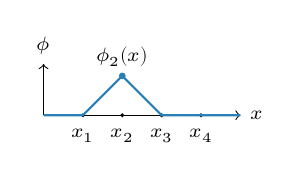
\begin{tikzpicture}[scale=0.50]
    % x-axis
    \draw[->] (0,0) -- (5,0) node[right] {\scriptsize $x$};
    \draw[->] (0,0) -- (0,1.3) node[above] {\scriptsize $\phi$};

    % Grid points
    \foreach \x in {1,2,3,4} {
        \filldraw[black] (\x,0) circle (1pt);
        \node[below] at (\x,-0.1) {\scriptsize $x_{\x}$};
      }

    % Hat function
    \draw[thick, primary] (0,0) -- (1,0) -- (2,1) -- (3,0) -- (5,0);
    \filldraw[primary] (2,1) circle (2pt);
    \node[above] at (2,1) {\scriptsize $\phi_2(x)$};
  \end{tikzpicture}
  \begin{formula}{Reference Elements}
    \textbf{Mapping from reference triangle $\hat{K}$ to physical element $K$:} \\
    $F_K(\hat{x},\hat{y}) =
      \begin{pmatrix} x_1 \\ y_1 \end{pmatrix} +
      \begin{pmatrix}
        x_2-x_1 & x_3-x_1 \\
        y_2-y_1 & y_3-y_1
      \end{pmatrix}
      \begin{pmatrix} \hat{x} \\ \hat{y} \end{pmatrix}$ \\[0.3em]
    \textbf{Jacobian of transformation:} \\
    $J_K = \det\begin{pmatrix}
        x_2-x_1 & x_3-x_1 \\
        y_2-y_1 & y_3-y_1
      \end{pmatrix}$ \\[0.3em]
    \textbf{Function transformation:} \\
    $\phi(x,y) = \hat{\phi}(\hat{x},\hat{y})$
  \end{formula}

  %----------------------------------------------------------------------------------------
  % FEM SECTION - APPLICATION
  %----------------------------------------------------------------------------------------

  \sheader{FEM Implementation Process}

  \begin{codebox}{Step-by-Step FEM Process}{fem-steps}
    1. \textbf{Define weak form}: Convert PDE to bilinear form \\
    2. \textbf{Create mesh}: Triangulate domain $\Omega$ \\
    3. \textbf{Choose finite element space}: $P_k$ elements \\
    4. \textbf{Assemble linear system}: \\
    \quad $K_{ij} = a(\phi_j,\phi_i)$ and $F_i = F(\phi_i)$ \\
    5. \textbf{Impose boundary conditions}: \\
    \quad Dirichlet: fix nodes directly \\
    \quad Neumann: include in weak form \\
    6. \textbf{Solve system}: $\mathbf{Ku} = \mathbf{F}$ \\
    7. \textbf{Post-process}: Compute error, visualize
  \end{codebox}

  \begin{formula}{Local Element Matrices}
    \textbf{For Poisson equation on a triangle $K$:} \\[0.3em]
    \textbf{Element stiffness matrix:} \\
    $A^K_{ij} = \int_K \nabla \phi_i \cdot \nabla \phi_j \, dK$ \\[0.3em]
    \textbf{Element mass matrix:} \\
    $M^K_{ij} = \int_K \phi_i \phi_j \, dK$ \\[0.3em]
    \textbf{Element load vector:} \\
    $F^K_i = \int_K f \phi_i \, dK$
  \end{formula}

  \begin{formula}{Quadrature Formulas}
    \textbf{1D:} $\int_0^1 f(x) \, dx \approx \sum_{q=1}^Q w_q f(x_q)$ \\[0.3em]
    \begin{tabular}{|c|c|c|c|}
      \hline
      \textbf{Rule} & \textbf{Points} & \textbf{Weights}  & \textbf{Order} \\
      \hline
      Midpoint      & $\{1/2\}$       & $\{1\}$           & 2              \\
      Trapezoidal   & $\{0,1\}$       & $\{1/2,1/2\}$     & 2              \\
      Simpson       & $\{0,1/2,1\}$   & $\{1/6,2/3,1/6\}$ & 4              \\
      \hline
    \end{tabular}\\[0.3em]
    \textbf{Triangle:} $\int_K f(x,y) \, dK \approx |K| \sum_{q=1}^Q w_q f(x_q,y_q)$
  \end{formula}

  \begin{formula}{Assembly Process}
    \textbf{1. Compute local matrices} $A^K$ for each element \\[0.3em]
    \textbf{2. Assembly by mapping local to global DOFs:} \\
    For each element $K$ with local nodes $i,j$: \\
    $A_{I(i),I(j)} \mathrel{+}= A^K_{ij}$ \\[0.3em]
    where $I(i)$ is global index of local node $i$ \\[0.3em]
    \textbf{3. Process boundary conditions:} \\
    Dirichlet: $A_{i,:} = 0, A_{i,i} = 1, b_i = g_i$ \\
    Neumann: Add boundary integral to $\mathbf{F}$
  \end{formula}

  %----------------------------------------------------------------------------------------
  % IMPORTANT THEOREMS AND LEMMAS
  %----------------------------------------------------------------------------------------

  \sheader{Key Theorems \& Results}

  \begin{formula}{Lax Equivalence Theorem}
    For consistent numerical schemes: \\
    \centerline{\alert{stability} $\Leftrightarrow$ \alert{convergence}}
  \end{formula}

  \begin{formula}{Lax-Milgram Theorem}
    If $V$ is a Hilbert space and $a:V \times V \rightarrow \mathbb{R}$ is: \\
    1. Continuous: $|a(u,v)| \leq M\|u\|_V\|v\|_V$ \\
    2. Coercive: $a(v,v) \geq \alpha\|v\|^2_V$ with $\alpha > 0$ \\
    Then for any bounded linear functional $F \in V'$: \\
    $\exists$ unique $u \in V$ such that $a(u,v) = F(v)$ $\forall v \in V$ \\
    Furthermore: $\|u\|_V \leq \frac{1}{\alpha}\|F\|_{V'}$
  \end{formula}

  \begin{formula}{Céa's Lemma}
    Let $V_h \subset V$ be a finite-dimensional subspace. Then: \\
    $\|u - u_h\|_V \leq C \inf_{v_h \in V_h} \|u - v_h\|_V$ \\
    where $C$ is a constant independent of $h$.
  \end{formula}

\end{multicols}
\end{document}
